\section{Delete Group}
\placeholder{Summary of delete group.}

\subsection{Parameters}
\begin{description}
    \item [groupID] The \texttt{GiD} of the group that is to be deleted.
\end{description}

\subsection{Results}
The group who's ID matches the given \texttt{groupID} will be deleted. If the group does not exist, nothing is displayed.

\begin{center}
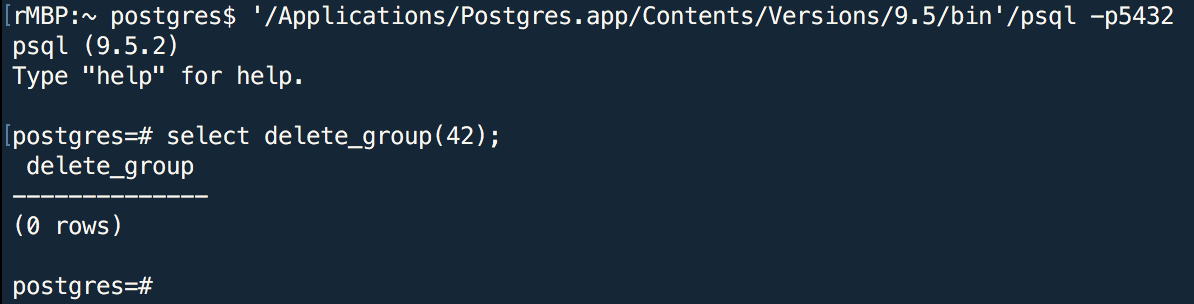
\includegraphics[width=\columnwidth]{include/assets/screenshots/delete_group}
\end{center}

% \section{Delete Group}
% Claire, something goes here.

% \subsection{Parameters}
% \begin{description}
%     \item [foo] bar
% \end{description}

% \subsection{Results}

% \begin{center}
% \includegraphics[width=\columnwidth]{}
% \end{center}